\documentclass[11pt,letterpaper]{article}
\usepackage[margin=1in]{geometry}
\setlength{\emergencystretch}{2em}
\usepackage[utf8]{inputenc}
\usepackage[T1]{fontenc}
\usepackage{mathtools}
\usepackage{amssymb}
\usepackage{amsthm}
\usepackage{microtype}
\usepackage{enumerate}
\usepackage{accents}
\usepackage{float}
\usepackage{tikz}
\usepackage{authblk}
\usepackage[colorlinks, pagebackref=true]{hyperref}
\hypersetup{
  linkcolor=[rgb]{0.3,0.3,0.6},
  citecolor=[rgb]{0.2,0.6,0.2},
  urlcolor=[rgb]{0.6,0.2,0.2},
  breaklinks=true
}
\usepackage{xurl}
\usepackage[capitalize, nameinlink]{cleveref}

\numberwithin{equation}{section}
% Keep the heading of a statement on the page of its first item.
\makeatletter
\@beginparpenalty=10000
% Reserve space before each statement, so that its hyperlink anchor moves with its heading.
\newcommand{\reservespace}{\par\penalty\z@\dimen@\pagegoal\advance\dimen@-\pagetotal
 \ifdim\dimen@<3\baselineskip\ifdim\dimen@>\z@\vfil\fi\break\fi}
\@for\@tempa:=theorem,lemma,corollary,definition\do{\AddToHook{env/\@tempa/before}{\reservespace}}
% Keep a heading together with at least five lines of what follows it.
\newcommand{\reservelines}[1]{\par\penalty\z@\dimen@\pagegoal\advance\dimen@-\pagetotal
 \ifdim\dimen@<#1\baselineskip\ifdim\dimen@>\z@\vfil\fi\break\fi}
\let\plainsection\section
\let\plainsubsection\subsection
\renewcommand{\section}{\reservelines{7}\plainsection}
\renewcommand{\subsection}{\reservelines{7}\plainsubsection}
\makeatother
\newtheorem{theorem}{Theorem}[section]
\newtheorem{lemma}[theorem]{Lemma}
\newtheorem{corollary}[theorem]{Corollary}
\theoremstyle{definition}
\newtheorem{definition}[theorem]{Definition}

\crefname{theorem}{Theorem}{Theorems}
\crefname{lemma}{Lemma}{Lemmas}
\crefname{corollary}{Corollary}{Corollaries}
\crefname{definition}{Definition}{Definitions}
\crefname{section}{Section}{Sections}
\crefname{subsection}{Section}{Sections}
\crefname{figure}{Figure}{Figures}

\DeclareMathOperator{\tensorrank}{R}
% Asymptotic rank.
\DeclareMathAccent{\wtilde}{\mathord}{largesymbols}{"65}
\DeclareMathOperator{\asymprank}{\underaccent{\wtilde}{R}}
\newcommand{\asympleq}{\lesssim}
\newcommand{\CC}{\mathbb{C}}
\newcommand{\FF}{\mathbb{F}}
\newcommand{\RR}{\mathbb{R}}
\newcommand{\QQ}{\mathbb{Q}}
\newcommand{\eps}{\varepsilon}
\newcommand{\mm}{\langle 2,2,2\rangle}
% Edges.
\newcommand{\se}{\mathsf e}
\newcommand{\sff}{\mathsf f}
% A compact convex set of functions on pairs of vertices.
\newcommand{\Cset}{\mathcal{C}}
% The number of partitions of the integers 0,...,n.
\newcommand{\PR}{\mathrm{PR}}
\newcommand{\psum}[1]{p_{\le#1}}

\title{Asymptotic rank via matrix multiplication\\ and sums of squares}
\author{Jeroen~Zuiddam}
\date{November 24, 2026}
\affil{University of Amsterdam}

\begin{document}
\maketitle

\begin{abstract}
We prove for every integer $n\ge1$ that every tensor in $\CC^n\otimes\CC^n\otimes\CC^n$ has asymptotic rank at most $n^{\omega/\sqrt3}$, where
$\omega$ is the matrix multiplication exponent. This improves the bound $n^{2\omega/3}$ of Strassen. Using
$\omega\le9/4$, this gives the bound $n^{3\sqrt3/4}\approx n^{1.29904}$. We generalise this to tensors in $\CC^{n_1} \otimes \CC^{n_2} \otimes \CC^{n_3}$. In particular, for tensors in $\CC^n\otimes\CC^n\otimes\CC^{n_3}$ with
$n^{4/\sqrt5}\le n_3\le n^2$ we show that the maximal asymptotic rank equals~$n_3$. 

We prove a dichotomy for asymptotic rank in terms of sums of squares. Let $\gamma$ be the
exponent of the least number of squares of complex bilinear forms with sum $(x_1^2+\cdots+x_m^2)(y_1^2+\cdots+y_m^2)$.
We prove that $\gamma$ is either~$1$ or~$\sqrt2$. If $\gamma=1$, then every tensor in
$\CC^n\otimes\CC^n\otimes\CC^n$ has asymptotic rank at most~$n^{\omega/2}$. If $\gamma=\sqrt2$, then there exist tensors in $\CC^m\otimes\CC^m\otimes\CC^m$ with
asymptotic rank at least $m^{2/\sqrt3-o(1)}$, which would refute the asymptotic rank conjecture.

\end{abstract}

\section{Introduction}\label{sec:intro}

Let~$\FF$ be a field. The asymptotic rank of a tensor~$T$ over~$\FF$ is $\asymprank(T)\coloneqq\lim_{m\to\infty}\tensorrank(T^{\otimes m})^{1/m}$, where
$\tensorrank$ is the tensor rank. Strassen~\cite[Lemma~3.5 and~(1.3)]{strassen1988asymptotic} showed for every integer
$n\ge1$ that every tensor in $\FF^n\otimes\FF^n\otimes\FF^n$ has asymptotic rank at most $n^{2\omega/3}$, where $\omega$ is the
matrix multiplication exponent over~$\FF$. The asymptotic rank conjecture~\cite{MR1341854}, \cite[Problem~15.5]{burgisser1997algebraic}, states that every tensor in
$\FF^n\otimes\FF^n\otimes\FF^n$ has asymptotic rank at most~$n$. For $\FF=\CC$, we make progress on this conjecture by proving a new
general bound on asymptotic rank in terms of the matrix multiplication exponent, using tensor networks, and by proving
a dichotomy in terms of a problem on sums of squares. More precisely:
\begin{itemize}
\item We prove for every integer $n\ge1$ that every tensor in $\CC^n\otimes\CC^n\otimes\CC^n$ has asymptotic rank at most $n^{\omega/\sqrt3}$.
Using $\omega\le9/4$, this gives the bound $n^{3\sqrt3/4}\approx n^{1.29904}$.
\item We extend this bound to all formats $\CC^{n_1}\otimes\CC^{n_2}\otimes\CC^{n_3}$, in terms of rectangular matrix
multiplication. In particular, for tensors in
$\CC^n\otimes\CC^n\otimes\CC^{n_3}$ with $n^{4/\sqrt5}\le n_3\le n^2$ we show that the maximal asymptotic rank is
exactly~$n_3$.
\item For every integer $m\ge1$, let $\sigma(m)$ be the smallest number~$s$ such that there are complex bilinear
forms $f_1,\ldots,f_s$ in $x,y\in\CC^m$ such that
\[
(x_1^2+\cdots+x_m^2)(y_1^2+\cdots+y_m^2)=f_1(x,y)^2+\cdots+f_s(x,y)^2.
\]
We prove that the limit $\gamma\coloneqq\lim_{m\to\infty}\log\sigma(m)/\log m$ exists, and that $\gamma$ is either~$1$
or~$\sqrt2$.
\item We prove the following: If $\gamma=1$, then for every integer $n\ge1$ every tensor in $\CC^n\otimes\CC^n\otimes\CC^n$ has
asymptotic rank at most $n^{\omega/2}$. If $\gamma=\sqrt2$, then there exist tensors in $\CC^m\otimes\CC^m\otimes\CC^m$ with asymptotic rank at least
$m^{2/\sqrt3-o(1)}$, which would refute the asymptotic rank conjecture.
\end{itemize}
All proofs in this paper were obtained with the large language models gpt-6.2-astra and Claude
Opus~5.5. The bound $n^{\omega/\sqrt3}$ was preceded by a long sequence of numerical
improvements of the exponent of the maximal asymptotic rank, obtained with several models. Theorems~\ref{thm:bound}, \ref{thm:formats}, \ref{thm:gap} and~\ref{thm:exponent} were obtained and
formalised in Lean on 21 November 2026, and Theorem~\ref{thm:formatdich} and Corollary~\ref{cor:334} on 24 November 2026. The results are
formalised in Lean~4 in \url{https://github.com/spectra-research/asymptotic-rank-omega-sqrt3}. We are preparing a full version of this paper with complete proofs.

In the rest of the text we explain the results in more detail.

\subsection{Asymptotic rank via the matrix multiplication exponent}\label{sec:intro-bounds}\label{sec:intro-context}

We discuss basic notions and then the results. We write $\log=\log_2$.

\subsubsection{Tensors, unit tensors, restriction, rank, asymptotic rank}

An element of
$V_1\otimes\cdots\otimes V_k$, for finite-dimensional vector spaces~$V_i$ over~$\FF$, we call a \emph{$k$-tensor}. We refer to the~$V_i$ as tensor legs. Let $e_1,\ldots,e_r$ be the standard basis of~$\FF^r$, let $\langle
r\rangle\coloneqq\sum_{i=1}^re_i\otimes\cdots\otimes e_i\in(\FF^r)^{\otimes k}$ be the \emph{unit tensor}.
A $k$-tensor $T\in V_1\otimes\cdots\otimes V_k$ is a \emph{restriction} of $S\in
U_1\otimes\cdots\otimes U_k$, written $T\le S$, if $T=(g_1\otimes\cdots\otimes g_k)S$ for linear maps $g_i\colon U_i\to
V_i$. The tensor product $S\otimes T\in\bigotimes_i(U_i\otimes V_i)$ groups the $i$th legs. The \emph{tensor rank}
$\tensorrank(T)$ is the smallest integer~$r$ such that $T\le\langle r\rangle$. The \emph{asymptotic rank} is
$\asymprank(T)\coloneqq\lim_{m\to\infty}\tensorrank(T^{\otimes m})^{1/m}$. For an integer $k\ge2$, distinct legs~$i$
and~$j$ and an integer $n\ge1$, let $\langle n\rangle_{ij}$ be the $k$-tensor $\sum_{x=1}^ne_x\otimes e_x$ on the
legs~$i$ and~$j$, tensored with $e_1\in\FF^1$ on every other leg.

\subsubsection{Matrix multiplication exponent}

For integers $n_1,n_2,n_3\ge1$, the \emph{matrix multiplication tensor} is
\[
 \langle n_1,n_2,n_3\rangle\coloneqq\sum_{a=1}^{n_1}\sum_{b=1}^{n_2}\sum_{c=1}^{n_3}(e_a\otimes e_b)\otimes(e_b\otimes
 e_c)\otimes(e_c\otimes e_a)\in\FF^{n_1n_2}\otimes\FF^{n_2n_3}\otimes\FF^{n_3n_1},
\]
where we identify $\FF^{p}\otimes\FF^{q}$ with~$\FF^{pq}$. We have
$\langle n_1,n_2,n_3\rangle \cong \langle n_1\rangle_{31}\otimes\langle n_2\rangle_{12}\otimes\langle
n_3\rangle_{23}$.  The \emph{matrix multiplication exponent} is
$\omega\coloneqq\log\asymprank(\langle2,2,2\rangle)$. By~\cite[(1.3)]{strassen1988asymptotic},
$\asymprank(\langle m,m,m\rangle)=m^\omega$ for every $m\ge1$.

\subsubsection{Maximal asymptotic rank and the \texorpdfstring{$2\omega/3$}{2omega/3} bound}

For every integer $n\ge1$, we define the maximal asymptotic rank of tensors in $\FF^n \otimes \FF^n \otimes \FF^n$ as
\[
 \asymprank[n]\coloneqq\sup\bigl\{\asymprank(T):T\in\FF^n\otimes\FF^n\otimes\FF^n\bigr\}.
\]
(For $\FF=\CC$ this supremum is actually attained~\cite[Theorem~1.2]{christandl2026asymptotictensorrankcharacterized}, but we will not need this.) Our starting point is the following simple upper bound on $\asymprank[n]$.

\begin{theorem}[Strassen~{\cite[Lemma~3.5 and~(1.3)]{strassen1988asymptotic}}]\label{thm:strassenbound}
For every integer $n\ge1$, $\asymprank[n]\le n^{2\omega/3}$.
\end{theorem}

\begin{proof}
Let $T\in\FF^n\otimes\FF^n\otimes\FF^n$. Then
\[
 T=\sum_{i,j,k=1}^nT_{ijk}\,e_i\otimes e_j\otimes e_k=\sum_{i,j=1}^ne_i\otimes e_j\otimes\Bigl(\sum_{k=1}^nT_{ijk}e_k\Bigr)
\]
for some $T_{ijk}\in\FF$. The linear map $\FF^{n^2}\to\FF^n$ with $e_j\otimes e_i\mapsto\sum_kT_{ijk}e_k$, on the third leg,
maps
\[
 \langle n,1,n\rangle=\sum_{i,j=1}^ne_i\otimes e_j\otimes(e_j\otimes e_i)\in\FF^n\otimes\FF^n\otimes\FF^{n^2}
\]
to~$T$, so $T\le\langle n,1,n\rangle$. Similarly, $T\le\langle1,n,n\rangle\in\FF^n\otimes\FF^{n^2}\otimes\FF^n$ and
$T\le\langle n,n,1\rangle\in\FF^{n^2}\otimes\FF^n\otimes\FF^n$. So $T^{\otimes3}\le\langle n,1,n\rangle\otimes\langle1,n,n\rangle\otimes\langle n,n,1\rangle\cong\langle n^2,n^2,n^2\rangle$. Asymptotic rank is
monotone under restriction and satisfies $\asymprank(T^{\otimes3})=\asymprank(T)^3$ by definition. Hence
$\asymprank(T)^3\le\asymprank(\langle n^2,n^2,n^2\rangle)=n^{2\omega}$.
\end{proof}

\subsubsection{Improved \texorpdfstring{$\omega/\sqrt3$}{omega/sqrt3} bound on asymptotic rank}

From now on, $\FF=\CC$. We improve the exponent $2\omega/3$ of \cref{thm:strassenbound} to $\omega/\sqrt3$.

\begin{theorem}\label{thm:bound}
For every integer $n\ge1$, $\asymprank[n]\le n^{\omega/\sqrt3}$.
\end{theorem}

Using $\omega\le9/4$~\cite[Theorem~1.1]{OAI:Matrix-Multiplication-Nine-Fourths-October-2-2026} (see
also~\cite{amanov2026multiplyingmatricespolynomialsexposition,dogan2026tensorvalue,li2026semidirect,shpilka2026exposition}), \cref{thm:bound} gives $\asymprank[n]\le n^{3\sqrt3/4}\approx n^{1.29904}$. The previous bound of \cref{thm:strassenbound}
gives $\asymprank[n]\le n^{3/2}$. The proof of \cref{thm:bound} uses the crossing decomposition
of~\cite{claude2026threeSAT,khoruzhii2026crossing}.

\subsection{Asymptotic rank of other formats via rectangular matrix multiplication}\label{sec:intro-formats}

For integers $n_1,n_2,n_3\ge1$, we define the maximal asymptotic rank of tensors in
$\CC^{n_1}\otimes\CC^{n_2}\otimes\CC^{n_3}$ as
\[
\asymprank[n_1,n_2,n_3]\coloneqq\sup\bigl\{\asymprank(T):T\in\CC^{n_1}\otimes\CC^{n_2}\otimes\CC^{n_3}\bigr\},
\]
so that $\asymprank[n]=\asymprank[n,n,n]$, and $\asymprank[n_1,n_2,n_3]$ is symmetric in $n_1,n_2,n_3$, since permuting the legs of~$T$ preserves $\asymprank(T)$. For reals $x_1,x_2,x_3\ge0$, we define the exponent of rectangular matrix multiplication as
\[
 \omega(x_1,x_2,x_3)\coloneqq\inf\bigl\{c\in\RR:\tensorrank(\langle\lceil n^{x_1}\rceil,\lceil n^{x_2}\rceil,\lceil
 n^{x_3}\rceil\rangle)=O(n^c)\text{ as }n\to\infty\bigr\}.
\]
It is symmetric, and $\omega(1,1,1)=\omega$.

For reals $a_1\le a_2\le a_3$ with $a_3<a_1+a_2$, there are points $Q_1,Q_2,Q_3\in\RR^2$ with $|Q_2-Q_3|=a_1$,
$|Q_1-Q_3|=a_2$ and $|Q_1-Q_2|=a_3$.

\begin{theorem}\label{thm:formats}
Let $1\le n_1\le n_2\le n_3$ be integers with logarithms $a_1\le a_2\le a_3$.
\begin{enumerate}[\upshape(i)]
\item\label{it:fmt-wide} If $a_3\ge a_1+a_2$, then $\asymprank[n_1,n_2,n_3]=n_1n_2$.
\item\label{it:fmt-bound} If $a_3<a_1+a_2$, then $\log \asymprank[n_1,n_2,n_3]$ is at most the infimum of
$\omega(|z-Q_1|,|z-Q_2|,|z-Q_3|)$ over $z\in\RR^2$.
\item\label{it:fmt-exact} If $a_3<a_1+a_2$ and there are reals $p,q\ge0$ with $p+q=a_3$ and
$a_3(pa_1^2+qa_2^2)\le pq(pq+a_3^2)$, then $\asymprank[n_1,n_2,n_3]=n_3$.
\item\label{it:fmt-square} In particular, $\asymprank[n,n,n_3]=n_3$ for all integers $n\ge1$ and~$n_3$ with $n^{4/\sqrt5}\le
n_3\le n^2$.
\end{enumerate}
\end{theorem}

\subsection{Exponent of the maximal asymptotic rank}\label{sec:intro-beta}

To illustrate the bounds of \cref{thm:strassenbound}, \cref{thm:bound} and \cref{thm:formats}, we define for reals
$x_1,x_2,x_3\ge0$ the exponent of the maximal asymptotic rank as
\[
 \beta(x_1,x_2,x_3)\coloneqq\limsup_{n\to\infty}\log_n\asymprank[\lceil n^{x_1}\rceil,\lceil n^{x_2}\rceil,\lceil
 n^{x_3}\rceil],
\]
and we let $\beta\coloneqq\beta(1,1,1)$. Since $\langle b,b,b\rangle\in(\CC^{b^2})^{\otimes3}$ has asymptotic
rank~$b^\omega$, we have $\beta\ge\omega/2$. Since $\asymprank[n^\ell]\ge\asymprank[n]^\ell$ for all integers $n,\ell\ge1$, the asymptotic rank conjecture states that $\beta=1$.

Since~$\asymprank[n_1,n_2,n_3]$ is nondecreasing in each argument, comparing the
dimensions for~$n$ with those for $\lceil n^t\rceil$ and $\lceil n^{1/t}\rceil$ shows that
$\beta(tx_1,tx_2,tx_3)=t\beta(x_1,x_2,x_3)$ for every real $t>0$. So \cref{fig:beta} shows $\beta(1,b,c)$ for $1\ge
b\ge c\ge0$.

The lower bound $\min(1,b+c)$ holds since some tensor in $\CC^{n_1}\otimes\CC^{n_2}\otimes\CC^{n_3}$ has rank
$\min(n_1n_2,n_3)$ as a matrix with rows indexed by the first two legs, and this matrix rank is multiplicative
under~$\otimes$ and at most the tensor rank. The upper bound is the bound of \cref{thm:formats}, which is
continuous and homogeneous of degree one in $a_1,a_2,a_3$, evaluated with the bound
of~\cite[Theorem~1.2]{amanov2026multiplyingmatricespolynomialsexposition} on $\omega(x_1,x_2,x_3)$ and with
$\omega\le9/4$.

If $\omega=2$, then $\omega(x_1,x_2,x_3)$ is the largest of $x_1+x_2$, $x_2+x_3$ and $x_3+x_1$. It is at least
this largest sum, since the three sums are the exponents of the dimensions of the three legs of $\langle\lceil n^{x_1}\rceil,\lceil
n^{x_2}\rceil,\lceil n^{x_3}\rceil\rangle$, and at most this largest sum, by cutting the matrices into square blocks of the
smallest side. So \cref{thm:formats}(\ref{it:fmt-bound}) with $z=(Q_1+Q_2)/2$ gives
$\asymprank[n_1,n_2,n_3]\le n_3$ if $a_1^2+a_2^2\le a_3^2<(a_1+a_2)^2$. With \cref{thm:formats}(\ref{it:fmt-wide}) for
$a_3=a_1+a_2$, this shows $\beta(1,b,c)=1$ if $b+c\ge1$ and $b^2+c^2\le1$.

In \cref{sec:intro-xm} we show, for the logarithms $a_1\le a_2\le a_3$ of integers with $a_3<a_1+a_2$, that
$\beta(a_1,a_2,a_3)$ is given by rectangular matrix multiplication if an exponent~$\gamma$ for sums of squares
equals~$1$, and we give a lower bound if $\gamma=\sqrt2$.

\begin{figure}[t]
\centering
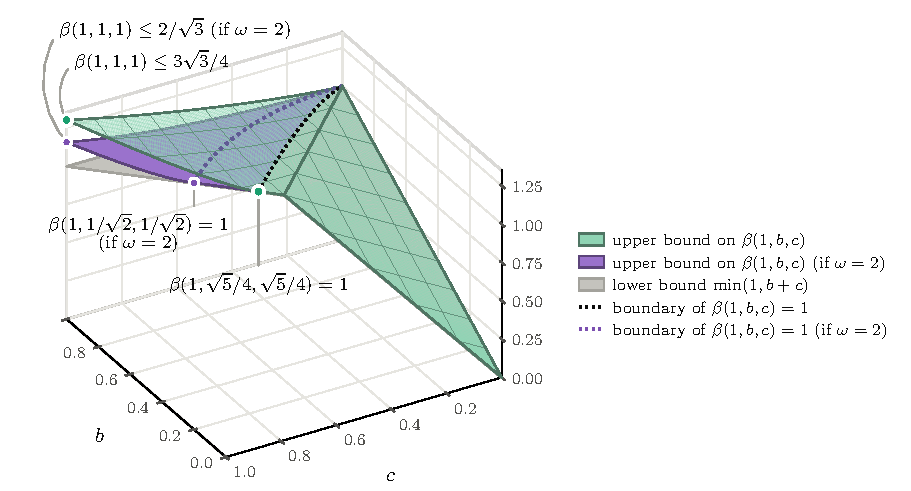
\includegraphics[width=\linewidth]{beta-figure.pdf}
\caption{Bounds on $\beta(1,b,c)$ for $1\ge b\ge c\ge0$. The green surface is the upper bound of \cref{thm:formats},
the purple surface the same bound if $\omega=2$, and the grey surface the lower bound $\min(1,b+c)$. The dotted curves
bound the region where we know that $\beta(1,b,c)=1$, by \cref{thm:formats} (black) and if $\omega=2$ (purple). The
dots mark $\beta(1,1,1)\le3\sqrt3/4$ (and $\le2/\sqrt3$ if $\omega=2$), $\beta(1,\sqrt5/4,\sqrt5/4)=1$, and
$\beta(1,1/\sqrt2,1/\sqrt2)=1$ if $\omega=2$.}\label{fig:beta}
\end{figure}

\subsection{Dichotomy for asymptotic rank in terms of sums of squares}\label{sec:intro-xm}

For every integer $m\ge1$ we study the $4$-tensor
\[
 \langle m\rangle_{13}\otimes\langle m\rangle_{24}=\sum_{a=1}^m\sum_{b=1}^me_a\otimes e_b\otimes e_a\otimes
 e_b\in\CC^m\otimes\CC^m\otimes\CC^m\otimes\CC^m.
\]

For a $k$-tensor~$T$ and a bipartition~$b$ of its legs, the \emph{flattening rank}~$\tensorrank_b(T)$ is the rank of~$T$
as a matrix with rows indexed by the legs in one part of~$b$ and columns by the legs in the other part. For bipartitions $b_1,\ldots,b_r$ of the legs, the \emph{restricted partition rank} $\PR_{b_1,\ldots,b_r}(T)$ of a
$4$-tensor~$T$ is the smallest number~$q$ such that there are $4$-tensors $S_1,\ldots,S_q$, each of flattening rank one
for one of $b_1,\ldots,b_r$, such that $T=S_1+\cdots+S_q$.
$\PR_{b_1,\ldots,b_r}$ is the $\{b_1,\ldots,b_r\}$-rank of Naslund~\cite[Definition~8]{MR4078997}. Grouping the terms by bipartition gives, for every $4$-tensor~$T$,
\[
 \PR_{12|34,14|23}(T)=\min\bigl\{\tensorrank_{12|34}(T_1)+\tensorrank_{14|23}(T_2):T=T_1+T_2\bigr\},
\]
over the $4$-tensors $T_1$ and~$T_2$.

For every integer $m\ge1$, let $\sigma(m)$ be the smallest number~$s$ such that there are complex bilinear forms
$f_1,\ldots,f_s$ in $x,y\in\CC^m$ such that
\[
 (x_1^2+\cdots+x_m^2)(y_1^2+\cdots+y_m^2)=f_1(x,y)^2+\cdots+f_s(x,y)^2.
\]

Hrube\v{s}, Wigderson and Yehudayoff~\cite{MR2784331} and Rossman and Zhu~\cite{rossman_et_al:LIPIcs.ITCS.2026.113}
related~$\sigma(m)$ to $\langle m\rangle_{13}\otimes\langle m\rangle_{24}$, and we use a version of their
relation.

We prove that the limit $\gamma\coloneqq\lim_{m\to\infty}\log_m\sigma(m)$ exists and that
\[
 \lim_{m\to\infty}\log_m\PR_{12|34,14|23}(\langle m\rangle_{13}\otimes\langle m\rangle_{24})=\gamma.
\]
Our main result about~$\gamma$ is that it can take only two values.

\begin{theorem}[Dichotomy]\label{thm:gap}
$\gamma\in\{1,\sqrt2\}$.
\end{theorem}

The next theorem bounds~$\beta$ in terms of~$\gamma$.

\begin{theorem}[Exponent dichotomy]\label{thm:exponent}\hfill
\begin{enumerate}[\upshape(i)]
\item\label{it:low} If $\gamma=1$, then $\beta=\omega/2$.
\item\label{it:high} If $\gamma=\sqrt2$, then $2/\sqrt3\le\beta\le\omega/\sqrt3$.
\end{enumerate}
\end{theorem}

Since $\beta\ge\omega/2$, and $2/\sqrt3>\omega/2$ by
$\omega\le9/4$, it follows that $\beta=\omega/2$
if and only if $\gamma=1$. If $\omega=2$, then $\beta=1$ if $\gamma=1$, and $\beta=2/\sqrt3$ if $\gamma=\sqrt2$. So
then the asymptotic rank conjecture holds if and only if $\gamma=1$.

The next theorem extends \cref{thm:exponent} to the formats of \cref{thm:formats}(\ref{it:fmt-bound}). A
$k$-tensor~$T$ is an \emph{asymptotic restriction} of a $k$-tensor~$S$, written $T\asympleq S$, if there are positive
integers $c_n=2^{o(n)}$ such that $T^{\otimes n}\le\langle c_n\rangle\otimes S^{\otimes n}$ for all $n\ge1$. Recall the
points $Q_1,Q_2,Q_3$ from \cref{sec:intro-formats}.

\begin{theorem}[Format dichotomy]\label{thm:formatdich}
Let $2\le n_1\le n_2\le n_3$ be integers with logarithms $a_1\le a_2\le a_3$ such that $a_3<a_1+a_2$, and let
$s\coloneqq(a_1+a_2+a_3)/2$.
\begin{enumerate}[\upshape(i)]
\item\label{it:fd-low} If $\gamma=1$, then $\beta(a_1,a_2,a_3)=\omega(s-a_1,s-a_2,s-a_3)$. If moreover
$n_1=b_{12}b_{13}$, $n_2=b_{12}b_{23}$ and $n_3=b_{13}b_{23}$ for integers $b_{12},b_{13},b_{23}\ge1$, then every
$T\in\CC^{n_1}\otimes\CC^{n_2}\otimes\CC^{n_3}$ satisfies $T\asympleq\langle b_{13},b_{12},b_{23}\rangle$.
\item\label{it:fd-high} If $\gamma=\sqrt2$, then $\beta(a_1,a_2,a_3)\ge2\rho$, where~$\rho$ is the smallest number~$r$
such that there is a point $z\in\RR^2$ with $|z-Q_i|\le r$ for $i=1,2,3$. If moreover $\omega=2$, then
$\beta(a_1,a_2,a_3)=2\rho$.
\end{enumerate}
\end{theorem}

For $n_1=n_2=n_3=2$, \cref{thm:formatdich} gives \cref{thm:exponent}(\ref{it:low}) and the lower bound of
\cref{thm:exponent}(\ref{it:high}). For an integer factorization as in part~(\ref{it:fd-low}), let
$M\coloneqq\langle b_{13},b_{12},b_{23}\rangle$. If $\gamma=1$, every tensor of this format is an asymptotic restriction
of~$M$. Since~$M$ itself has this format, $\asymprank[n_1,n_2,n_3]=\asymprank(M)$.

Since $\omega(2,2,1)=4$ by~\cite[Theorem~1.1]{uznanski2026rectangularmatrixmultiplicationpolynomial} (see also~\cite[Theorem~1.2]{amanov2026multiplyingmatricespolynomialsexposition}),
\cref{thm:formatdich} for $(n_1,n_2,n_3)=(8,8,16)$ gives a criterion for~$\gamma$ that, unlike the one after
\cref{thm:exponent}, does not depend on the value of~$\omega$.

\begin{corollary}\label{cor:334}
The following three statements are equivalent.
\begin{enumerate}[\upshape(i)]
\item\label{it:334-gamma} $\gamma=1$.
\item\label{it:334-beta} $\beta(3,3,4)=4$.
\item\label{it:334-rank} $\asymprank[t^3,t^3,t^4]=t^4$ for every integer $t\ge1$.
\end{enumerate}
If $\gamma=\sqrt2$, then $\beta(3,3,4)\ge9/\sqrt5\approx4.02492$.
\end{corollary}

\paragraph{Acknowledgements.} JZ was supported by NWO Vidi grant VI.Vidi.243.195, by ERC Starting Grant 101220349 SPECTRA, and by the Simons Institute for the Theory of Computing, UC Berkeley, as part of the 2025 semester programme Complexity and Linear Algebra. This work used the Dutch national e-infrastructure with the support of the SURF Cooperative using grant no.~EINF-16525.

\bibliographystyle{alphaurl}
\bibliography{results}
\end{document}
